\chapter{Proposed Model} 
\label{chapter:proposed_model}

Population mobility area studies the large-scale flow of a population in a given geographic space, describing this population as a whole instead of its individuals~\cite{brockmann2006scaling,gonzalez2008understanding}. This approach may have different degrees of granularity, as populations can be studied in a given district, city, state, country, continent, or even the entire world and in different time scales, as data can be hourly, daily, monthly, yearly, and so on. 
In this work, we propose LodusPop, a flexible framework for multi-scale population simulation. Instead of representing individuals or fixed groups, LodusPop models populations as variable-sized units, each with defined characteristics and behavioral patterns. This design enables seamless adjustment of simulation detail, adapting to both the availability of data and the requirements of the study.

The simulation process relies on data to function effectively. LodusPop can utilize real-world datasets while offering the flexibility to customize population parameters. Indeed, LodusPop was designed to simulate population mobility allowing the integration of data from diverse sources, such as real-world datasets and programmed scripts. 
Figure~\ref{fig:data_diagram} illustrates the potential data sources and their integration within the components of our proposed model.
On the left, we can see possible sources of data, which are specified in the center, that can be used in the platform. On the right, the core components of LodusPop are depicted: the environment, defining the simulated space; the population, representing entities moving within the environment; and the simulation behavior, responsible for generating actions that influence the population. These components are detailed in the subsequent sections. 
As an example, a simulation designer can define a population and model their behavior using a combination of real-world and synthetic datasets. Environmental data can be sourced from Geographic Information Systems (GIS) databases like OpenStreetMap. Population profiles may be derived from census data (Real Population) or generated synthetically (Synthetic Population) to fit the specific needs of an experiment. Additionally, data describing population behavior, such as routines, can be obtained from sources like Origin-Destination Matrices, GPS tracking services, or user-generated inputs.

\begin{figure}[ht]
 \centering
  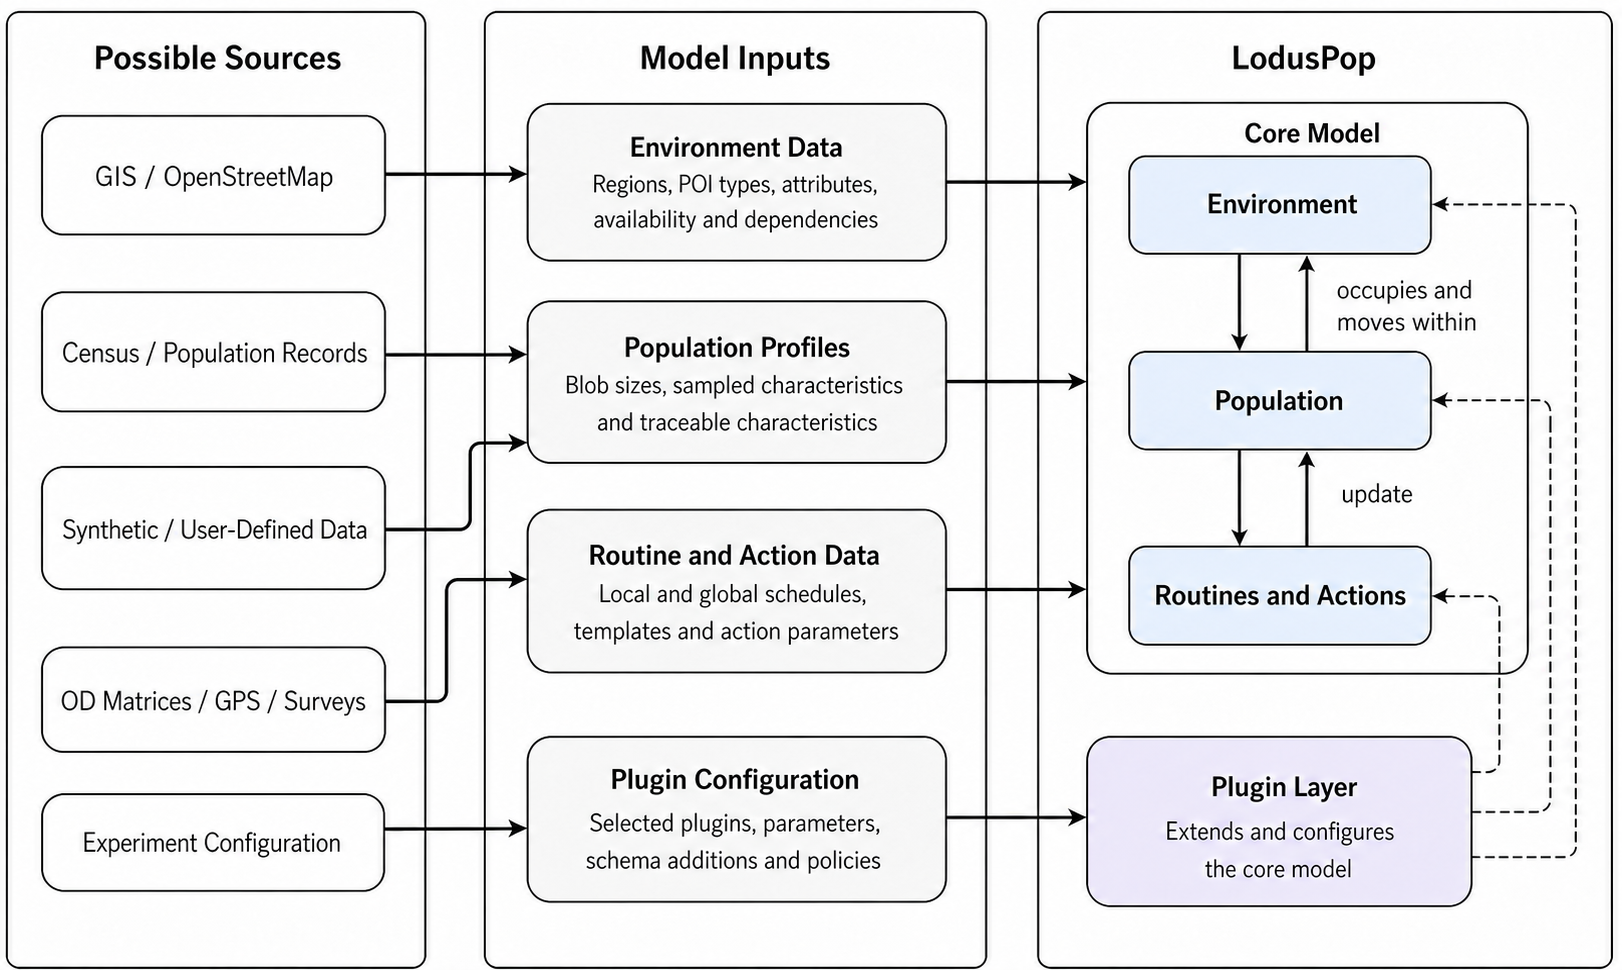
\includegraphics[width=0.98\textwidth]{fig/model/DataDiagram.png}
  \caption{Flowchart illustrating the integration of data sources into the LodusPop framework. Inputs such as GIS databases, census data, user-generated data, and GPS tracking services are processed into geographic data, population characteristics, and behavioral routines. In our proposed model, routines consist of actions that influence population behavior, driving their movement through the environment.
  }
  \label{fig:data_diagram}
\end{figure}


Population mobility frameworks typically operate across multiple spatial scales, such as neighborhoods, cities, and states. In this work, we seek to integrate strategies from crowd simulation into human mobility modeling, particularly the ability of macroscopic models to abstract individual behaviors~\cite{thalmann2007crowd, treuille2006continuum}. To achieve this, we propose representing populations as blobs—aggregated groups of individuals of varying sizes. In this context, Blob is an abstract structure, similar to a cloud or a legion~\cite{antonitsch2019bioclouds}, but designed to represent larger and more heterogeneous populations. Unlike BioClouds and Legion, which assume homogeneous population clusters, our blobs can encompass diverse individual and group attributes and evolve within environments containing locations that demand specific population profiles.

Furthermore, our environment design builds upon the approach proposed by Silva et al.~\cite{silva2020lodus}. However, our model introduces greater flexibility, allowing regions of the simulated environment to represent different semantic entities beyond the fixed hierarchy of countries, states, regions, and cities, enabling more adaptable and context-specific representations.

In LodusPop, we can define a set of characteristics for each blob, representing a population of a specific profile distributed in the environment and changing temporally and spatially in the simulation. For instance, one group, representing a blob, might consist of children going to school in the morning and returning home in the afternoon, illustrating spatial movement within a city. Another example involves changes in population parameters, such as healthy workers commuting to their jobs in the morning, with some individuals becoming sick during the day, resulting in healthy individuals returning home and sick individuals heading to a hospital, in this case representing a split in the blob structure.

Our proposed model considers the following elements to provide population simulation, which will be described in the next sections. 
\begin{itemize}
    \item a) An environment modeled as a graph of regions and points of interest that the population can occupy;
    \item b) The population is modeled as blobs that can split and merge and can contain characteristics of the population; and
    \item c) a set of population movement actions and routines to describe the desired population behavior during the simulation.
\end{itemize} 

\section{Environment}
\label{sec:environment}

To adequate our population mobility simulation to different spatial scopes, we model the environment as an abstract graph composed of \textit{regions} and \textit{points of interest}. The regions ($R$) represent areas of physical space in the virtual world that can contain points of interest ($P$), which represent locations that motivate human travel and that can have population groups (i.e., blobs $B$).
When setting up a simulation, users define the spatial scope that $R$ and $P$ represent. For example, in a city simulation, $R$ could correspond to districts, while $P$ might represent markets, malls, hospitals, residential buildings, and commercial centers.



\begingroup\color{red}
A region $R$ is represented as a finite set of points of interest $\{P_1,\ldots,P_m\}$. Each point of interest combines a semantic description of the location, its current population, its local behavior, and its availability conditions. We represent $P_i$ as

\begin{equation}
P_i=\bigl(\tau_i,\bm{\alpha}_i,\bm{B}_{P_i},Ro_{P_i},C_i(t),D_i\bigr),
\label{eq:poi_definition}
\end{equation}

where $\tau_i$ is its type, $\bm{\alpha}_i$ is its attribute mapping, $\bm{B}_{P_i}$ contains the blobs currently located at $P_i$, $Ro_{P_i}$ is its local routine, $C_i(t)$ contains its direct disable causes at step $t$, and $D_i$ specifies its dependency constraints.

The type $\tau_i$ identifies the semantic role of the location, such as \textit{home}, \textit{work}, \textit{school}, \textit{hospital}, or \textit{water source}. Types allow actions and plugins to select locations that perform the same role without enumerating them individually. 
%Atributos não tinhamos no paper
The attribute mapping $\bm{\alpha}_i:K_i\rightarrow V_i$ is a mutable finite dictionary of key--value pairs. It stores location-specific information such as coordinates, capacity, an external identifier, or a flood-exposure threshold. Plugins may declare expected keys and may add, access, or modify their values. An attribute has no framework-wide behavioral meaning unless the core model or a loaded plugin defines how it is interpreted.

% Texto adaptado do que já tinhamos no paper
The components $\bm{B}_{P_i}$ and $Ro_{P_i}$ describe the relationship between the location and the simulated population. The former contains the blobs currently occupying $P_i$, while the latter specifies the actions generated by that location over time. 
These components support the inversion of responsibility that characterizes LodusPop. In many agent-based approaches, populations decide where to go based on individual preferences or probabilistic rules. Even in field-based models, agents typically remain responsible for sampling and following environmental fields. 
In LodusPop, locations instead request populations with particular characteristics. Moving part of the decision logic from individuals to points of interest and regions reduces dependence on granular individual-level movement data and permits aggregated or generalized descriptions of population demand.

For example, a market $P_m$ may use $Ro_{P_m}$ to request consumers, while $\bm{B}_{P_m}$ represents the population currently at the market. Similarly, a school $P_j$ may request students, and a hospital $P_k$ may request patients. In each case, the routine expresses the population demanded by the location and the contained blobs represent the population currently occupying it.

In addition to describing occupation and behavior, a point of interest records whether it is available to participate in simulation actions. Let $C_i(t)$ be the set of direct causes disabling $P_i$ at step $t$, such as an off-cycle
closure or flood exposure. A point of interest in available exactly when $C_i(t)$ is empty. A point of interest may also depend on the availability of other locations. Its dependency specification is 
%and let $q_i(t)=1$ exactly when $C_i(t)$ is empty. A point of interest may also depend on the availability of other locations. Its dependency specification is

\begin{equation}
D_i=\left(D_i^{\mathrm{all}},D_i^{\mathrm{min}}\right),
\qquad D_i^{\mathrm{min}}=\{(k_g,G_g)\},
\label{eq:poi_dependencies}
\end{equation}

where every point of interest in $D_i^{\mathrm{all}}$ must be available and each pair $(k_g,G_g)$ requires at least $k_g$ available points of interest from $G_g$. The first form represents mandatory dependencies, while the second
represents groups of substitutable prerequisites. 

% Equação abaixo sugerida pelo GPT com base no que foi implementado em código.
\begin{comment}

Let $q_i(t)=1$ exactly when $C_i(t)$ is empty. The effective availability of $P_i$ is
\begin{equation}
e_i(t)=q_i(t)\land
\bigwedge_{P_j\in D_i^{\mathrm{all}}}e_j(t)\land
\bigwedge_{(k_g,G_g)\in D_i^{\mathrm{min}}}
\left[\sum_{P_j\in G_g}e_j(t)\geq k_g\right].
\label{eq:poi_availability_redline}
\end{equation}
When no dependency rule is declared, $e_i(t)=q_i(t)$.   
\end{comment}

Dependencies may be transitive, so effective states are recomputed until no state changes. Removing one cause from $C_i(t)$ cannot enable the point of interest while another cause or an unsatisfied dependency remains. This avoids, for example, reopening a flooded facility merely because its scheduled closure ended.

Availability records whether a location can participate in an action; it does not prescribe a universal population response. A plugin may suppress a request from a disabled origin, reject a disabled destination, retain demand in a queue, select a fallback, or reroute it. These alternatives are domain policies and remain outside the core environment definition.

\endgroup

Figure~\ref{fig1:environment} illustrates
regions, typed points of interest, contained blobs, and routines in a LodusPop
environment.
Table~\ref{tbl:notation_env} summarizes the notation introduced in this section.
Additionally, Appendix~\ref{app:input} outlines the process of defining the input data necessary for designing a simulation. Appendix~\ref{app:input_environment} specifically addresses the data required to model the simulation environment. 

\begin{figure}[ht]
 \centering
  
\includegraphics[width=0.98\textwidth]{fig/model/Environment.png}
  \caption{A diagram of a LodusPop environment. The figure presents two regions, $R_i$ and $R_j$, containing different points of interest $P$. Each point of interest may contain groups of the population (i.e., blobs), and routines are responsible for moving them in the environment during the simulation.}
  \label{fig1:environment}
\end{figure}


\begin{table}[ht]
\footnotesize
\centering
\caption{Mathematical notation and descriptions of the elements defined in Section~\ref{sec:environment}.}
\label{tbl:notation_env}
\begin{tabularx}{\linewidth}{@{}lcX@{}}
\toprule
\textbf{Element} & \textbf{Notation} & \multicolumn{1}{c}{\textbf{Description}} \\ \midrule
Region & $R$ & Represent areas of physical space in the virtual world that can contain points of interest. A region $R_i$ is defined as a set of $P$. \\ \midrule
\begin{tabular}[c]{@{}l@{}}Point of\\ Interest\end{tabular} & $P$ & Represent locations that the population can occupy as they move during a simulation. \change{A $P_i$ is defined by its type ($\tau_i$), an attribute mapping ($\bm{\alpha}_i$), a collection of population blobs ($\bm{B}_{P_i}$), its local routine ($Ro_{P_i}$), its direct disable causes ($C_i(t)$), and dependency constraints ($D_i$).} \\ \midrule
\change{POI type} & \change{$\tau_i$} & \change{Semantic role used to identify locations of the same kind, such as home, work, or school.} \\ \midrule
\change{POI attributes} & \change{$\bm{\alpha}_i$} & \change{Mutable key--value mapping through which plugins add, access, and modify location-specific information.} \\ \midrule
\change{Direct disable causes} & \change{$C_i(t)$} & \change{Named, independently removable causes that directly prevent $P_i$ from being available at step $t$.} \\ \midrule
\change{Dependency constraints} & \change{$D_i$} & \change{All-of and minimum-of prerequisite rules used to derive effective availability.} \\ %\midrule
%\change{Effective availability} & \change{$e_i(t)$} & %\change{Boolean state obtained from direct causes and the effective states of all prerequisites.} \\ 
\bottomrule
\end{tabularx}
\end{table}

\FloatBarrier

\section{Population}
\label{sec:population}

\begingroup\color{red}
The population in LodusPop is represented by an abstraction of people into blobs $B$, each located at one point of interest at any given simulation step. Blobs describe population groups rather than tracking individuals. A point of interest becoming unavailable does not, by itself, remove or relocate its blobs; any cancellation, waiting, relocation, or redirection of population is performed explicitly by an action according to the policy of the core model or a loaded plugin.

Formally, a blob is denoted by
\begin{equation}
B=(TP,\bm{Tc},\bm{Sc}),
\label{eq:blob_definition}
\end{equation}
where $TP$ is its total number of individuals, $\bm{Tc}$ is its collection of traceable characteristics, and $\bm{Sc}$ is its collection of sampled characteristics. Table~\ref{tbl:notation_pop} summarizes this notation and the associated terminology.

Sampled characteristics in $\bm{Sc}$ represent distributions within the blob. For example, the sampled characteristic \textit{Age} may contain the categories \textit{Child}, \textit{Adult}, and \textit{Elder}, each associated with a number of individuals. Multiple sampled characteristics can jointly describe distributions such as age, schooling level, and employment status.

Traceable characteristics in $\bm{Tc}$ instead store one value for the entire blob. For instance, if \textit{Vaccination status} can be \textit{Vaccinated} or \textit{Unvaccinated}, every individual represented by a particular blob has the same value for that characteristic. The traceable-characteristic schema is simulation-specific. 
% Cola com plugins, talvez remover?
During initialization, a plugin may extend it through $\Delta\Sigma_{\Pi}$ by declaring a characteristic and its default value (Section~\ref{sec:plugins}). The default is applied consistently to the population, after which the characteristic can be read or modified by actions and used as a predicate in population templates.
\endgroup

These characteristics allow us to specify the population in more detail, e.g., elderly people who are currently vaccinated against a given disease or the number of adults who commute to work by bus. Following the previous examples, it becomes possible to track vaccination by age group in the simulation by identifying all blobs $B$ with a \textit{Vaccinated} status and their respective \textit{Age} distributions. Figure~\ref{fig2:blob_diagram} shows a diagram of a blob, including its characteristics and associated distributions. Appendix~\ref{app:input_population} presents an example of the input data required to model the initial population in simulations.

\begingroup\color{red}
During the simulation, actions generated by the local routine $Ro_{P_i}$ may operate on the blobs contained in $P_i$. An action can target a particular population profile, such as children traveling from $P_i$ to a school $P_j$, by applying a population template to the sampled category $Age=Child$.

A population template $T$ specifies which individuals are eligible for an action and the requested quantity. We represent it as

\begin{equation}
T=(T_Q,\bm{T_{Tc}},\bm{T_{Sc}}),
\label{eq:population_template_definition}
\end{equation}

where $T_Q$ is the requested quantity, $\bm{T_{Tc}}$ is an optional set of predicates on traceable characteristics, and $\bm{T_{Sc}}$ is an optional set of predicates on sampled characteristics. Applied to one or more blobs, $T$ filters the eligible population and selects up to $T_Q$ individuals satisfying all declared predicates. Because $\bm{T_{Tc}}$ refers to the active traceable-characteristic schema, it may include characteristics introduced by loaded plugins.
\endgroup


\begin{figure}[ht]
 \centering
  
\includegraphics[width=0.9\textwidth]{fig/model/BlobDiagram.png}
  \caption{Diagram of a Blob $B_A$ containing 100 people, three traceable characteristics, and three sampled characteristics. Traceable characteristics describe the entire blob population and can have any value type. The distribution of each sampled characteristic sum should be equal to the total population of the blob.} 
  \label{fig2:blob_diagram}
\end{figure}


Consider a blob $B_j$ with two sampled characteristics: \textit{i)} \textit{Age}, which includes the possible values \textit{Children}, \textit{Adults}, and \textit{Elders}, and \textit{ii)} \textit{Occupation}, with possible values \textit{Student} and \textit{Worker}. A template $T$ that specifies \textit{Age=Adults} in its collection of sampled characteristics will target only the specified group within $B_j$, in this case, only adults. If the template $T$ does not include a filter for the second sampled characteristic (Occupation), all occupation categories in $B_j$ are affected. The number of affected individuals in categories such as Students and Workers is determined proportionally based on their distribution within $B_j$. For instance, if $B_j$  contains more students than workers, a larger proportion of students will be selected. This process continues until the total number of individuals defined in $T$ is selected or until there are no remaining eligible individuals in $B_j$.

% Splits
When a blob is operated using a population template $T$, it is possible that only a portion of its population may be affected, e.g., a blob $B_i$ that has 75 people and only 20 are selected in $T$. If the operation is to move to another $P$, then such 20 people will create a new blob. This operation generates a split, i.e., the original blob will be separated into two smaller ones. 
In such an example, a template with quantity $T_Q = 20$ selects 20 people from $B_i$ and splits it by creating a new blob $B_j$, which is moved to a different $P$. 
The same occurs when modifying a blob's $\bm{Tc}$s. For example, another blob $B_k$ has 90 \textit{Healthy} people, 
and 20 are selected, using $T$, to be infected by a disease. The split occurs, and a \textit{InfectionStatus} of $B_l$ (newly created blob) is changed to \textit{Infected}.

% Merge
\begingroup\color{red}
In addition to split operations, compatible blobs can be merged by combining their total populations $TP$. 
Each sampled characteristic of the resulting blob is obtained by summing the corresponding category counts of the merged blobs. A merge can occur only between blobs in the same point of interest that have equal values for every active traceable characteristic, including characteristics introduced by plugins. Consequently, adding a traceable characteristic may also refine the groups that remain distinguishable during merging.
\endgroup
% Figure
Figure~\ref{fig3:blob_operations_with_template} presents a diagram of blobs affected by two templates, resulting in splits and merges. The first scenario, depicted at the top of the figure, demonstrates the relocation of a population. 
The second scenario illustrates changes in traceable characteristics of a population.


\begin{figure}[ht]
 \centering
  
\includegraphics[width=0.99\textwidth]{fig/model/BlobOperations.png}
  \caption{
  Diagram presenting two scenarios of blobs being modified. The first scenario (1) (on the top) shows a population being moved to another location. In 1a, the initial blob $B_i$ has a population of 100. In 1b, a template $T$ selects 30 people, splitting $B_i$ and creating $B_j$. In 1c, $B_j$ is moved to $P_j$. The second scenario (2) shows a population's traceable characteristics changed. In 2a, there are two blobs, $B_i$ containing 100 unvaccinated people (in red), and $B_j$ containing 50 vaccinated people (in green). In 2b, a template $T$ selects 20 unvaccinated people, affecting only $B_i$ and splitting it into $B_k$. In 2c, the traceable characteristic \textit{VaccStatus} of $B_k$ is changed to \textit{Vaccinated}. In 2d, $B_k$ is merged into $B_j$ since they now share the same characteristics and are in the same $P_i$.
  } 
  \label{fig3:blob_operations_with_template}
\end{figure}

\begin{table}[h]
\footnotesize
\centering
\caption{Mathematical notation and descriptions of the elements defined in Section~\ref{sec:population}.}
\label{tbl:notation_pop}
\begin{tabularx}{\linewidth}{@{}lcX@{}}
\toprule
\textbf{Element}                                                             & \textbf{Notation} & \multicolumn{1}{c}{\textbf{Description}}                                                                                                                                                                                                                                                                                     \\ \midrule
Blob                                                               & $B$        & \change{Population abstraction $B_i=(TP_i,\bm{Tc}_i,\bm{Sc}_i)$, comprising a total population, traceable characteristics, and sampled characteristics.} \\ \midrule
\begin{tabular}[c]{@{}l@{}}Traceable\\ Characteristic\end{tabular} & $Tc$       & \change{Identifier--value pair shared by the entire blob. Plugins may declare additional traceable characteristics and defaults during initialization.} \\ \midrule
\begin{tabular}[c]{@{}l@{}}Sampled\\ Characteristic\end{tabular}   & $Sc$       & Characteristic with a categorical distribution over the blob population. Defined as a string identifier and a collection of its possible categories, each associated with a certain number of people. \\ \midrule
\begin{tabular}[c]{@{}l@{}}Population\\ Template\end{tabular}      & $T$        & \change{Filter $T=(T_Q,\bm{T_{Tc}},\bm{T_{Sc}})$ specifying an eligible population profile and requested quantity for an action.} \\ \bottomrule
\end{tabularx}
\end{table}

\FloatBarrier

\section{Routines and Actions}
\label{sec:routines}

\begingroup\color{red}
Behavioral dynamics in LodusPop are expressed through routines and plugin hooks, which schedule actions at discrete simulation steps. We consider a simulation organized into cycles of fixed length $d$. Within each cycle, the cycle step is indexed by $t\in\{0,\ldots,d-1\}$, while $s$ denotes the absolute simulation step used by plugins and data services.

A routine is an ordered finite sequence of scheduled actions,

\begin{equation}
Ro=\langle(t_1,A_1),\ldots,(t_n,A_n)\rangle.
\label{eq:routine_definition}
\end{equation}

The ordering is significant when two or more actions share the same cycle step. For each point of interest $P_i$, the local routine $Ro_{P_i}$ describes actions requested by that location. The global routine $GRo$ has the same structure and schedules actions across the environment rather than belonging to one point of interest. Plugins may contribute entries to either routine and may additionally produce start-of-step or end-of-step actions through $\mathcal{R}_{\Pi}$.

Every action retains the common representation

\begin{equation}
A=(N,T,\bm{V}),
\label{eq:action_definition}
\end{equation}

where $N$ identifies the action type, $T$ is a population template, and $\bm{V}$ contains the additional parameters required by that action. The handler registered for $N$ determines how $T$ and $\bm{V}$ are interpreted. For population-targeting actions, $T$ selects the eligible individuals; an action that does not select population may ignore an empty template. Table~\ref{tbl:notation_rout} summarizes this notation.
\endgroup

In the core implementation, LodusPop provides two built-in action types:
\textit{move population} (MOV), which moves a subset of a blob between points of interest; and \textit{change traceable characteristic} (CH), which modifies the traceable characteristics of a subset of a blob.

A MOV action expects its parameter vector $\bm{V}$ to specify an origin and a destination point of interest. For example, the local routine of $P_i$ may include the pair $(t = 15, A)$, where $A = (MOV, T_i, \\bm{V}_i)$, with $T_i=(T_Q=20, T_{Tc}=\emptyset, T_{Sc}=\{Age=Child\})$, and $\bm{V}_i$ encoding $P_i$ as origin and $P_j$ as destination. At cycle step $t = 15$, this action selects 20 children from the blobs at $P_i$, splits them into a new blob, and moves that blob to $P_j$.

A CH action expects $\bm{V}$ to contain the name of a traceable characteristic and its new value. For instance, the local routine of $P_j$ may include $(t = 25, A')$, with $A' = (CH, T_j, \bm{V}_j)$, where $T_j=(T_Q=20, T_{Tc}=\{Status=Unvaccinated\}, T_{Sc}=\emptyset)$, and $\bm{V}_j$ encodes the update ``Status := Vaccinated''. At cycle step $t=25$, this action selects 20 unvaccinated individuals from the blobs at $P_j$, splits them into a new blob, and changes the traceable characteristic Status of that blob to Vaccinated. Figure~\ref{fig3:blob_operations_with_template} illustrates both the movement and characteristic-change scenarios.



% Global routines and Queueing
\begingroup\color{red}
The same action representation is used by the global routine $GRo$. For example, MOV or CH entries in $GRo$ may schedule effects across all points of interest at cycle step $t$, enabling global phenomena such as random walks or disease spread. These actions share a scheduling step but are consumed sequentially, not simultaneously. Appendix~\ref{app:input_routine} provides an example of the input data used to encode local and global routines.
\endgroup

% Movido para a nova seção de plugins
%New action types with Plugins 
%New action types can be added via plugins. A plugin registers an additional identifier $N$ together with a function that consumes actions of that type. Plugin actions retain the same structure $A=(N,T,V)$. The simulation still uses the population template $T$ to select the affected individuals and passes $T$ and $\bm{V}$ to the plugin’s function. Appendix~\ref{app:plugin} illustrates how plugins can be used to introduce custom action types into simulations.

\begingroup\color{red}
To produce repeating temporal behavior, the simulation iterates over cycle steps $t=0,\ldots,d-1$. At each absolute step $s$, actions are processed in the following phases:
\begin{enumerate}
    \item simulation lifecycle and plugin hooks are updated, and start-of-step actions are generated and consumed;
    \item actions scheduled for cycle step $t$ by $GRo$ and each $Ro_{P_i}$ are collected and consumed in their defined order;
    \item end-of-step actions contributed by plugins are generated and consumed; and
    \item after all actions have completed, one merge pass combines compatible blobs at each point of interest.
\end{enumerate}

The simulator dispatches each action according to its identifier $N$. A primitive handler applies its state transition directly. A composite plugin handler may instead emit an ordered sequence of core or plugin actions, which is recursively consumed through the same action contract before execution continues with the next scheduled action. Each population-targeting action evaluates its template against the state produced by all preceding actions. Thus, the same blob or its descendants may be affected more than once during a step, and later actions observe earlier splits, movements, and characteristic changes.

POI availability does not alter this execution contract. The handler consuming an action determines whether an unavailable origin or destination causes that action to be suppressed, queued, redirected, or otherwise transformed. Figure~\ref{fig:simulation_diagram} illustrates the simulation behavior over one cycle, and Appendix~\ref{app:simulator} presents an example of the overall simulation control flow.
\endgroup

\begin{figure}[ht]
 \centering
  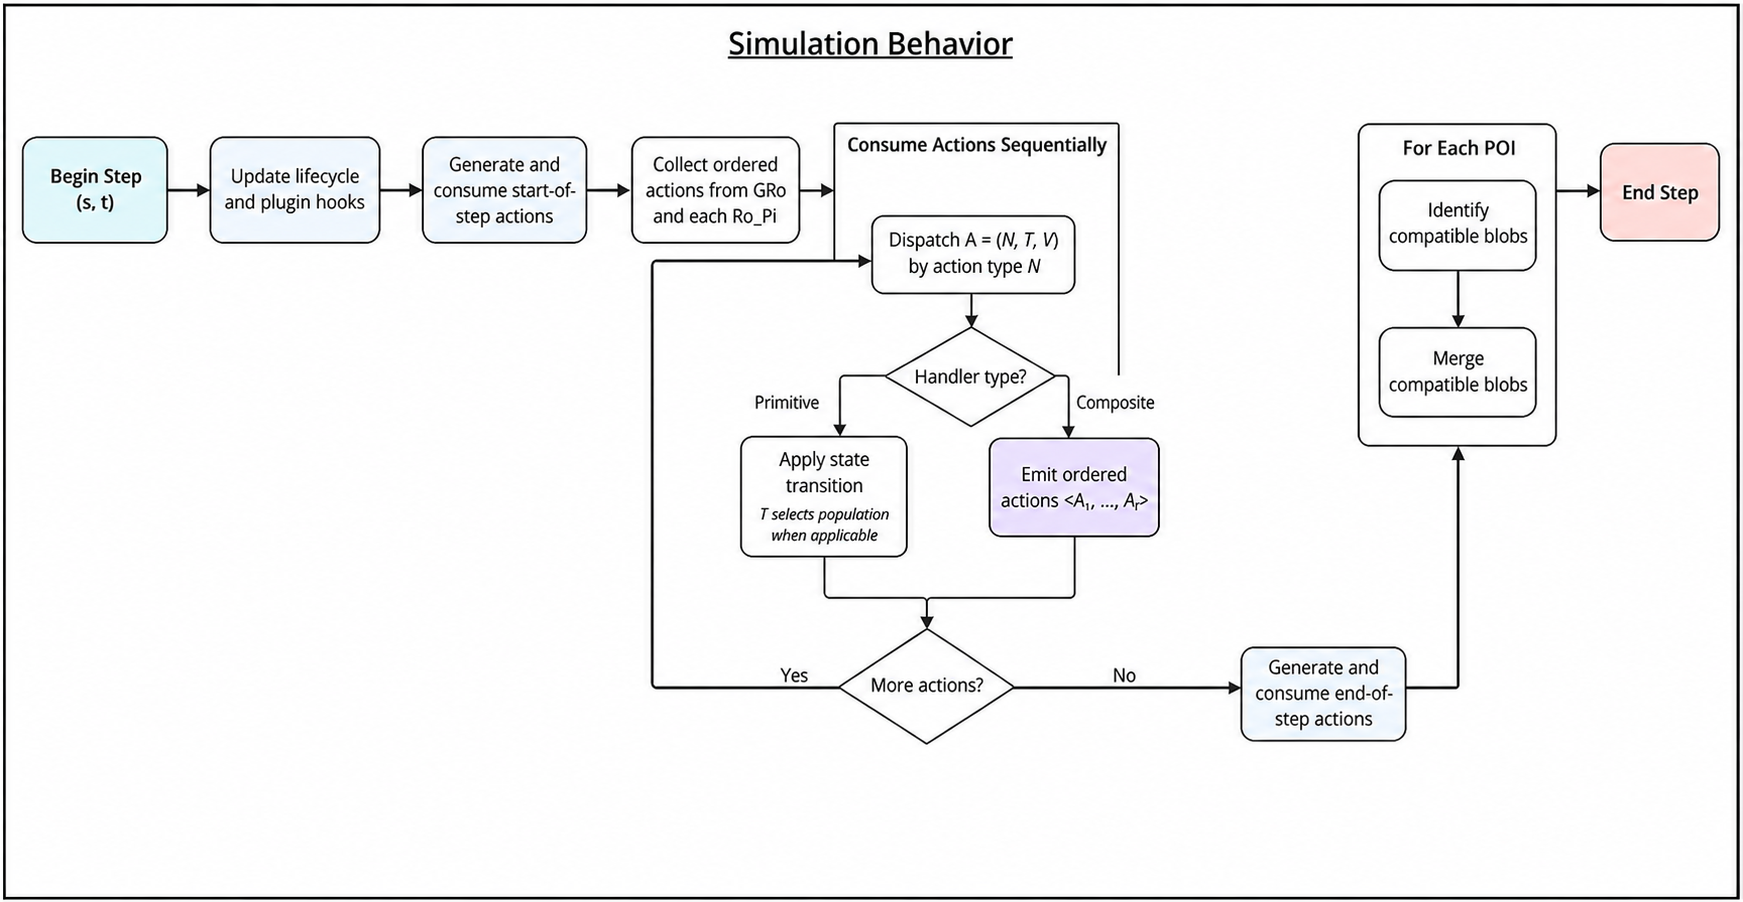
\includegraphics[width=0.99\textwidth]{fig/model/SimulationBehaviorDiagram.png}
  \caption{\change{Diagram of the simulation behavior, illustrating the identification and sequential execution of actions from global and local routines. Plugin-contributed start-of-step and end-of-step actions follow the same action contract. A primitive action may modify blobs directly, while a composite action may emit further actions; subsequent actions operate on the resulting state. After all phases of the step have completed, compatible blobs in each point of interest are merged.}}
  \label{fig:simulation_diagram}
\end{figure}




\begin{table}[ht]
\footnotesize
\centering
\caption{Mathematical notation and descriptions of the elements defined in Section~\ref{sec:routines}.}
\label{tbl:notation_rout}
\begin{tabularx}{\linewidth}{@{}lcX@{}}
\toprule
\textbf{Element} & \textbf{Notation} & \multicolumn{1}{c}{\textbf{Description}} \\ \midrule
\begin{tabular}[c]{@{}l@{}}Local\\ Routine\end{tabular} & $Ro_{P_i}$ & \change{Ordered finite sequence of scheduled actions associated with $P_i$, represented by $\langle(t_1,A_1),\ldots,(t_n,A_n)\rangle$.} \\ \midrule
\begin{tabular}[c]{@{}l@{}}Global\\ Routine\end{tabular} & $GRo$ & \change{Ordered routine with the same structure as a local routine, used to schedule actions across the environment.} \\ \midrule
Action & $A$ & \change{Action $A_i=(N_i,T_i,\bm{V}_i)$ comprising a type identifier, a population template, and additional parameter values. The handler registered for $N_i$ defines their interpretation.} \\ \bottomrule
\end{tabularx}
\end{table}

\change{The core action types establish the population-transition semantics shared by all LodusPop simulations. Domain-specific actions, routines, state updates, and observations are introduced through plugins, described in the following section.}


\FloatBarrier

\section{Plugins}
\label{sec:plugins}

\change{Toda essa section (Plugins) é nova.}

The core model defines the structures and execution rules shared by every simulation, whereas plugins provide the behavior required by a particular application domain. Plugins extend rather than replace points of interest, blobs, population templates, routines, and actions. An experiment selects a set of plugins and supplies their parameters in its experiment file. Depending on its role, a plugin may add traceable characteristics and their defaults, define conventions for point-of-interest attributes, contribute routines, register new action types, invoke or emit other actions, expose data services, or record outputs.

Let $\mathcal{S}(s)$ denote the complete simulation state at simulation step $s$, including points of interest, blobs, routines, availability states, and action registries. 
A plugin is defined through the extension contract

% Notação sugerida por IA com base na implementação de plugins
\begin{equation}
\Pi=\left(\bm{\theta}_{\Pi},\Delta\Sigma_{\Pi},\mathcal{R}_{\Pi},
\mathcal{F}_{\Pi},\mathcal{H}_{\Pi}\right),
\label{eq:plugin_definition}
\end{equation}

where:
\begin{itemize}
    \item $\bm{\theta}_{\Pi}$ is a finite key--value mapping of parameters read from the experiment configuration;
    \item $\Delta\Sigma_{\Pi}$ contains optional additions to the model vocabulary, including declarations and defaults for traceable characteristics and point-of-interest attribute conventions;
    \item $\mathcal{R}_{\Pi}$ is an optional finite collection of local or global routine contributions;
    \item $\mathcal{F}_{\Pi}=\{(N,f_N)\}$ is an optional registry associating action-type identifiers with the handlers that consume them; and
    \item $\mathcal{H}_{\Pi}$ contains optional lifecycle, time-step,
    data-access, observation, and logging hooks.
\end{itemize}

Any component may be empty, and a plugin need only use the extension points required by its role. %The notation consequently covers action, routine, logger, and data plugins without requiring each plugin to implement every mechanism.

At load time, the simulator reads $\bm{\theta}_{\Pi}$, applies the declarations in $\Delta\Sigma_{\Pi}$, incorporates $\mathcal{R}_{\Pi}$, registers $\mathcal{F}_{\Pi}$, and activates $\mathcal{H}_{\Pi}$. 
During execution, each registered pair $(N,f_N)$ associates an action identifier $N$ with the handler that consumes actions of that type. 
Plugin actions retain the common action structure $A=(N,T,\bm{V})$, so their handlers receive the same population template and additional values used by core actions. At a high level, a handler is described as

\begin{equation}
f_N:\bigl(\mathcal{S}(s),T,\bm{V},t,s;\bm{\theta}_{\Pi}\bigr)
\longmapsto
\bigl(\mathcal{S}'(s),\langle A_1,\ldots,A_\ell\rangle\bigr).
\label{eq:plugin_action_handler}
\end{equation}

% Ações simples e complexax
A primitive handler applies its transition directly to $\mathcal{S}$ and may return an empty action sequence. A composite handler may instead return core or plugin-defined actions, which are consumed through the same $A=(N,T,\bm{V})$ contract. This makes calls to other actions explicit while preserving population-template selection and sequential execution.

The lifecycle and observation hooks in $\mathcal{H}_{\Pi}$ allow a plugin to update the simulation at step boundaries, expose data to other plugins, record state, and release its resources. 
% Abaixo, plugins que dependem de outros plugins
A loaded set of plugins $\mathbb{P}=\{\Pi_1,\ldots,\Pi_r\}$ is valid when its action identifiers and schema declarations are compatible and all plugin requirements are present.
%Dependencies between plugins must be stated by the experiment; for example, a mobility plugin may require an action type provided by a population-gathering plugin. 
%Appendix~\ref{app:plugin} illustrates the implementation of such an extension.

The same definition provides a reporting template for the experimental chapters:

\begin{equation}
\Pi_x=(\bm{\theta}_x,\Delta\Sigma_x,\mathcal{R}_x,
\mathcal{F}_x,\mathcal{H}_x).
\label{eq:experiment_plugin_template}
\end{equation}

An experiment need only describe the nonempty components and the scenario values of $\bm{\theta}_x$. For example, a dialysis plugin can state its capacity and service parameters in $\bm{\theta}_x$, patient-state characteristics in $\Delta\Sigma_x$, scheduled requests in $\mathcal{R}_x$, and service handlers and update hooks in $\mathcal{F}_x$ and $\mathcal{H}_x$.

% Diferença de informações de POIs vs Plugins acessando e modificando o comportamento base
Point-of-interest state and plugin behavior remain distinct. The tuple $P_i$ defines where location data are stored and how effective availability is derived. The tuple $\Pi$ defines the experiment-specific rules that read or modify that state and determine the population response. 
For example, a flood plugin may compare a forcing value with a threshold in $\bm{\alpha}_i$ and add a cause to $C_i(t)$. The dependency constraints $D_i$ then propagate effective unavailability, after which a mobility or service plugin decides whether the resulting demand is canceled, queued, or redirected. Service capacities, queues, flood thresholds, patient stays, destination substitution, and commute lifecycles consequently remain explicit plugin policies rather than universal fields of every blob or point of interest.

\begin{table}[ht]
\color{red}
\footnotesize
\centering
\caption{Mathematical notation and descriptions of the plugin extension contract.}
\label{tbl:notation_plugins}
\begin{tabularx}{\linewidth}{@{}lcX@{}}
\toprule
\textbf{Element} & \textbf{Notation} & \multicolumn{1}{c}{\textbf{Description}} \\ \midrule
Plugin & $\Pi$ & Extension contract $(\bm{\theta}_{\Pi},\Delta\Sigma_{\Pi},\mathcal{R}_{\Pi},\mathcal{F}_{\Pi},\mathcal{H}_{\Pi})$. \\ \midrule
Configuration & $\bm{\theta}_{\Pi}$ & Experiment-supplied parameter mapping. \\ \midrule
Schema additions & $\Delta\Sigma_{\Pi}$ & Population characteristics, defaults, and POI-attribute conventions introduced by the plugin. \\ \midrule
Routine contributions & $\mathcal{R}_{\Pi}$ & Local, global, start-of-step, or end-of-step actions contributed by the plugin. \\ \midrule
Action registry & $\mathcal{F}_{\Pi}$ & Pairs $(N,f_N)$ associating action identifiers with consuming handlers. \\ \midrule
Hooks and services & $\mathcal{H}_{\Pi}$ & Lifecycle, time-step, data-access, observation, and logging interfaces. \\ \bottomrule
\end{tabularx}
\end{table}


%\FloatBarrier

% ---------------------------------------------------------------------------
% Definições alternativas para plugins (sugestões de IA)
% ALTERNATIVE PLUGIN DEFINITION 2 (compact transition-operator view)
% This option treats a configured plugin as one operator over state and pending
% actions. It is compact, but hides which extension mechanisms an experiment uses.
% \[
% \Pi_{\bm{\theta}}:\mathcal{S}\times A^{*}\longrightarrow
% \mathcal{S}\times A^{*}.
% \]
% The operator may transform state, consume actions, and emit actions. Setup,
% routine injection, logging, and schema changes would require separate prose.

% ALTERNATIVE PLUGIN DEFINITION 3 (base-model delta view)
% This option defines a plugin by the changes it contributes to a base simulator.
% It emphasizes composition, but is less convenient for parameters and stateful
% hooks in an experimental specification.
% \[
% \Pi=(\Delta\Sigma,\Delta Ro,\Delta F,\Delta H),
% \qquad M_{\Pi}=M_0\oplus\Pi.
% \]
% Here \Delta\Sigma extends the schema, \Delta Ro extends routines, \Delta F
% extends the action registry, and \Delta H extends lifecycle and observation
% hooks. Parameters would be supplied separately as \Pi_{\bm{\theta}}.
% ---------------------------------------------------------------------------
